
\documentclass[a4paper,12pt]{article}
\date{}

%-----------------------------------------------------------------------------
% Language setting, set page size and margins
%-----------------------------------------------------------------------------
\usepackage[english]{babel}
\usepackage[a4paper,top=2.5cm,bottom=2.5cm,left=2.5cm,right=2.5cm,marginparwidth=1.75cm]{geometry}
\usepackage{setspace}
\onehalfspacing %interligne 1.5
%----------------------------------------------------------------------------

% Useful packages
\usepackage{amsmath}
\usepackage{amssymb}
\usepackage{graphicx}
\usepackage[hidelinks]{hyperref}
%\usepackage[colorlinks=true, allcolors=blue]{hyperref}

%----------------------------------------------------------------------------
% Packages: uncomment to debug
%----------------------------------------------------------------------------
\usepackage{refcheck}
\renewcommand{\labelitemi}{\textbullet}

%----------------------------------------------------------------------------
% Packages: bibliography
%----------------------------------------------------------------------------
\usepackage[nottoc, notlof, notlot]{tocbibind}
%\usepackage[square,sort,comma,numbers]{natbib}
\usepackage[authoryear]{natbib}
%\usepackage[english]{babel}
\usepackage{authblk}

%----------------------------------------------------------------------------
% Acronyms
%----------------------------------------------------------------------------
\usepackage[acronyms]{glossaries}
\makeglossaries
%\newacronym{Identifiant unique}{Nom de l’acronyme}{Définition de l’acronyme}
\newacronym{kh}{KH}{Kelvin-Helhmoltz}

%----------------------------------------------------------------------------
% Page de garde
%----------------------------------------------------------------------------
\usepackage[utf8]{inputenc}
\usepackage[T1]{fontenc}
%\usepackage{fullpage}
\usepackage{eso-pic}
\newcommand{\HRule}{\rule{\linewidth}{0.5mm}}
\newcommand{\blap}[1]{\vbox to 0pt{#1\vss}}
\newcommand\AtUpperLeftCorner[3]{%
  \put(\LenToUnit{#1},\LenToUnit{\dimexpr\paperheight-#2}){\blap{#3}}%
}
\newcommand\AtUpperRightCorner[3]{%
  \put(\LenToUnit{\dimexpr\paperwidth-#1},\LenToUnit{\dimexpr\paperheight-#2}){\blap{\llap{#3}}}%
}

\title{ \Large{Rapport de Stage M2 SOAC-DC}}
\author{Marie Andrieux}
\makeatletter

%----------------------------------------------------------------------------
%----------------------------------------------------------------------------
%----------------------------------------------------------------------------
%                           BEGIN DOCUMENT
%----------------------------------------------------------------------------
%----------------------------------------------------------------------------
%----------------------------------------------------------------------------

\begin{document} 
%\maketitle
\thispagestyle{empty}

%----------------------------------------------------------------------------
% \ref with ( )
%----------------------------------------------------------------------------
\let\noparref\ref
\renewcommand{\ref}[1]{(\noparref{#1})}


%----------------------------------------------------------------------------
% Page de garde
%----------------------------------------------------------------------------
\begin{titlepage}
    \enlargethispage{2cm}
 
    \AddToShipoutPicture{
        %\AtUpperLeftCorner{1.5cm}{1cm}{\includegraphics[width=4cm]{figures/logolegos.jpg}}
        %\AtUpperRightCorner{1.5cm}{1cm}{\includegraphics[width=6.5cm]{data/logola.jpg}}
        }
 
    \begin{center}
        \vspace*{10cm}
        \textsc{\@title} \\
        \newline
        \large{\bf Influence de la diffusion moléculaire sur le mélange de traceurs passifs}
        \HRule
        \vspace*{0.5cm}
        \large{\@author} \\
        \newline
        \small{Tuteurs: Yves Morel (Legos), Francis Auclair (Laero) et Cyril Nguyen (Laero)}
        
    \end{center}
 
    \vspace*{9.2cm}
 
    \begin{center}
        %\makebox[\textwidth]{\includegraphics[width=\paperwidth]{figures/???}}
    \end{center}
 
\end{titlepage}
\ClearShipoutPicture

\newpage
%----------------------------------------------------------------------------
% Page numbering
%----------------------------------------------------------------------------
\renewcommand{\thepage}{\arabic{page}}
\setcounter{page}{1}


%----------------------------------------------------------------------------
%%  ABSTRACT
%----------------------------------------------------------------------------
\begin{abstract}
25 à 30 pages maximum dont le contenu indicatif est le suivant : 1 résumé, 1 table des matières, 1 liste des acronymes si nécessaire, 1 introduction (posant la problématique, restituant les questions abordées dans leur contexte scientifique ou industriel, et présentant la démarche utilisée/suivie pour aborder cette thématique), 1 description de la méthodologie, 1 présentation des résultats ou des cas d’étude, 1 discussion, 1 conclusion avec des perspectives, 1 conclusion personnelle d’une demi-page précisant les
apports du stage (pour le rapporteur de l'université, pas nécessairement dans le rapport à l'encadrant), bibliographie.  Le rapport peut être rédigé en anglais ou en français.
- Possibilité de mettre des annexes (utiles pour l’équipe d’accueil/l’entreprise) qui ne seront pas évaluées et dont la lecture ne doit pas être indispensable à la compréhension du rapport. - Format impératif du rapport : police caractères taille 12, marges 2,5 cm, interligne 1.5.
\end{abstract}

%----------------------------------------------------------------------------
%%  TABLE DES MATIERES
%----------------------------------------------------------------------------
\newpage
\tableofcontents

%\newpage
%\printglossary[type=\acronymtype]

%----------------------------------------------------------------------------
%%  ACRONYMES
%----------------------------------------------------------------------------
\newpage
Liste des acronymes \\
Remerciements\\

%----------------------------------------------------------------------------
%%  INTRODUCTION
%----------------------------------------------------------------------------
\newpage
\section{Introduction}

    %\subsection{Problématique}
    \textbf{\textit{Le mélange dans l'océan}} \\
    Contexte, c'est quoi le mélange, comment il agit dans l'océan, quel est son impact ? \\
    Le mélange est l'action d'homogénisation d'un volume fluide. Dans le cas de l'océan il correspond à la redistribution de propriétés de masse d'eau comme la chaleur, la salinité, les espèces chimiques et biologiques. \\
    Mais comme ce mélange agis à l'échelle de la particule fluide les temps d'homogénisation sont long d'autant plus que les volimes sont grands. Une cascade turbulente permet de descendre dans ces petites échelle et de produire un mélange efficace qui peut avoir un impact rapide sur des échelles macroscopiques. \\
    Le forcage turbulent peut être de nature différente (cisaillement, tension du vent, convection, frottement de fond). \\
    Impacts sur l'océan: circulation générale, polluant, plancton, ... \\
    %\subsection{Instabilité de Kelvin-Helmholtz}
    \newline
    \textbf{\textit{De l'instabilité de Kelvin-Helmholtz vers la cascade turbulente}} \\
    Cascade turbulente \\
    Transfère d'énergie vers les petites échelles \\
    == diffusion moléculaire \\
    KH : cisaillement - stratification \\
    Nombre de Richardson \\
    Nombre de Reynolds \\
    Théorie de Taylor-Golstein \\
    ... \\
    ... \\
    Instabilités convectives, transverses \\
    Diffusion moléculaire efficace \\
    (Spectre d'énergie turbulente) \\
    Instabilité de \acrfull{kh} \\
    %\subsection{Démarche}
    \newline
    \textbf{\textit{Approche utilisée}} \\
    Démarche utilisée, modélisation directe et analyse physique

%----------------------------------------------------------------------------
%%  METHODE
%----------------------------------------------------------------------------
\newpage
\section{Méthode}

%--Modèle Croco--------------------------------------------------------------
    \subsection{Le modèle CROCO-NBQ}
    
    Les simulations présentées ici ont été réalisées avec le modèle CROCO (Coastal and regional ocean community) en version non-Boussinesq et non-hydrostatique.
    CROCO est un modèle dédié à l'océan, notamment à la modélisation de l'échelle régionale, issu du code numérique ROMS (Regional ocean modeling system) auquel a été ajouté les effets compressibles et non-hydrostatiques (\citep{auclair_non-hydrostatic_2018}). \\
    \newline
    NBQ (Non-Boussinesq) signifie qu'on ne fait pas l'approximation de Boussinesq qui est une approximation classique en physique de l'océan. Elle consiste à supposer que la densité de l'eau de mer varie peu dans l'espace et dans le temps autour d'une valeur moyenne $\rho(x,y,z,t)=\rho_{0}+\rho'(x,y,z,t)$. Cette hypothèse permet de négliger les variations de densité dans les équations de Navier-Stokes à l'exception du terme de gravité. Or dans notre étude, nous avons besoin de ces termes de variation de densité puisqu'on étudie le mélange diapycnal. \\
    \newline
    Non-hydrostatique :\\
    L'approximation hydrostatique est aussi une approximation classique en physique de l'océan, car elle est basée sur le fait que les longueurs horizontales des bassins sont très grandes devant les longueurs verticales. Les termes d'accélérations verticales sont donc négligés ce qui mène à l'équilibre hydrostatique. Or ici, nous avons besoin de cette accélération verticale pour créer des instabilités. \\
    \newline
    (Quasi-) Compressible :\\ 
    La compressibilité autorise les ondes acoustiques à se propager. Dans nos études, les ondes acoustiques ne sont pas essentielles, mais dans CROCO, elles sont un moyen de réduire le coût numérique des simulations. Elles sont associées à un sous pas de temps ($\Delta t_{FAST}$) --> évite une équation de poisson très coûteuse. \\
    Dans l'océan, les ondes acoustiques se propagent normalement à une vitesse de $c_s \approx 1500 m.s^{-1}$. Mais ici, nous avons seulement besoin qu'elles fassent un aller-retour dans tout le domaine avant un pas de temps "lent". On peut donc diminuer la vitesse de propagation des ondes acoustiques qui est réduite à un paramètre numérique... \\
    \newline
    Condition de bords :\\
     \\
    \newline
    Pas de fermeture turbulente :\\

%--Analyse physique----------------------------------------------------------------
    \subsection{Analyse physique}
    
        \subsubsection{Diagramme de dispersion}
        
        Pour suivre le mélange diapycnal, les propriétés des particules fluides peuvent être représentées dans un espace 2D avec en coordonnées la concentration en traceur et la densité. 
        Ce diagramme de dispersion met en évidence les changements de caractéristiques de particules. En effet, une particule fluide reste à la même position dans ce diagramme quelque soit son déplacement ou sa déformation géométrique dans l'espace physique. En revanche, si les propriétés sont modifiées par un mélange irréversible dans l'espace physique, la distribution des particules fluides changera dans ce diagramme de dispersion. 
        Des diagrammes similaires sont souvent utilisés pour caractériser le mélange dans les flux géophysiques, tels que les diagrammes température-salinité utilisés pour quantifier le mélange de grandes masses d'eau dans l'océan (par exemple \citep{tomczak_multi-parameter_1981}) ; les courbes de mélange traceur-salinité dans une embouchure, utilisées pour déterminer si un estuaire peut agir comme source ou puits d'un traceur donné (par exemple, \citep{loder_dynamics_1981} et \cite{officer_dynamics_1981}); ou des diagrammes de traceurs-traceurs utilisés pour examiner les relations compactes entre différents traceurs atmosphériques (par exemple, \cite{tilmes_development_2006} et \cite{plumb_tracer_2007}). Les diagrammes de dispersion sont donc pratiques pour l'analyse présentée ici, car ils permettent l'identification directe du mélange de traceur dans des nouvelles gammes de densités
        %transport de traceurs diapycnal 
        qui doit être indiqué par la génération de nouveaux points dans l'espace densité-traceur.\\
        %\newline
        Pour mieux représenter la distribution en densité et traceur, chaque point dans cet espace est associé a un "poids" qui est une formulation discrète de la fonction de probabilité densité-traceur présentée à l'annexe D de \cite{plumb_tracer_2007}. Le poids de chaque point quantifie sa concentration en densité ou traceur, il est représenté par l'échelle de couleur sur les figures. \\
        \newline
        \cite{penney_diapycnal_2020} ont montré que si l'évolution de la densité et du traceur est gouvernée par une équation d'advection-diffusion et que les coefficients de diffusion moléculaire de densité et de traceur passif sont égaux, il existe une contrainte sur l'évolution de ce diagramme. \cite{plumb_tracer_2007}, \cite{lauritzen_evaluating_2012} ont déjà utilisé cette méthode pour déterminer si le mélange dans les modèles numériques est physique. 
        + Figure 8 de Jared.
    
    
        \subsubsection{Réarrangement isopycnal}
        
        Le réarrangement isopycnal est un formalisme pour visualiser l'évolution macroscopique de l'instabilité en trouvant, de manière conservative, un profil vertical 1D à partir du domaine 3D. Il a été introduit par \citep{nakamura_two-dimensional_1996} et \citep*{winters_diascalar_1996} pour des écoulements spatialement inhomogènes où les traceurs sont advectés et diffusés. \\
        \newline
        Article Jared : \textit{Contours (in two dimensions) or surfaces (in three dimensions) of tracer concentration are used to define coordinate surfaces or contours, but the latter are labelled not by the value of the tracer concentration but the area (in two dimensions) or volume (in three dimensions) enclosed by the surface. If the tracer has some kind of geometric organisation, then the coordinate system and the variation of tracer concentration within that system represent that organisation. For the KH instability and for other flows in density-stratified fluids, the natural tracer is the density and the corresponding tracer-based coordinate, z\∗, represents a vertical coordinate. \\
        Note that the rearranged (or background) density field ρ∗(z∗, t) may be calculated from the 3-D simulation by rearrangement to construct a monotonic profile. That is, fluid elements, each with a specified infinitesimal volume, are ordered by their density, giving density as a function of cumulative volume (i.e. the volume of fluid with density less than a given value), and then the volume is converted to a vertical coordinate z∗ by dividing by the horizontal area of the fluid domain. The coordinate z∗ is then a decreasing function of ρ∗. The value of z∗ for a given ρ∗ is therefore proportional to the integral, down to ρ∗ of the weight defined previously in § 4.1. (Note that, typically, (5.1) is written in terms of ρ and z∗ (for example, Smyth et al. 2005), with ∂ρ/∂z∗ implicitly referring to the adiabatic rearrangement of the density field. For clarity, ρ∗ will be used here for density when it is being regarded as a function of z∗, and ρ will be used when it is being regarded as a function of the Cartesian coordinates (x, y,z), such as in the numerator of the right-hand side of (5.2).)}
        \newline
        Ce réarrangement isopycnal est en faite une représentation macroscopique des processus petites-échelles. Il a l'avantage d'être conservqtif, c'est-à-dire de ne pas modifier les propriétés des particules, le terme de réarrangement adiabatiques est souvent utilisé dans la litterature. C'est le seul moyen connu d'obtenir un profil macroscopique sans rajouter de processus non-conservatif (diabatique) contrairement a une moyenne spatiale qui, par définition, homogénise les propriétés sur un espace donné. \\
        Le profil obtenu issu du réarrangement de la densité est le profil de plus basse énergie potentiel et il ne varie au cours du temps qu'avec des processus non-conservatif i.e avec le mélange (\cite*{winters_diascalar_1996}. --> extraction du mélange diffusif et convectif (pour des fluides incompressibles winter et d'asaro)
        
        
        \subsubsection{Diffusion effective}
        
        La diffusion effective est la diffusion efficace à l'échelle macroscopique. Or l'évolution du profil macroscopique (issu du réarrangement isopycnal) peut être écrite sous la forme d'une équation de diffusion (\citep{penney_diapycnal_2020-1}): 
        \begin{equation}
            \label{rho*}
            \frac{\partial\rho_*}{\partial t}=\frac{\partial}{\partial z_*}(K_{\rho}\frac{\partial\rho_*}{\partial z_*})
        \end{equation}
        Avec $K_{\rho}$ la diffusion effective, seule inconnue de cette équation, l'évolution de $\rho_*$ nous est donné par le réarrangement isopycnal du résultats de la simulation. D'après l'appendix C de \citep{penney_diapycnal_2020-1}, la diffusion effective s'écrit sous la forme :
        \begin{equation}
            \label{Keff}
            \frac{K_{\rho}}{\kappa_{\rho}}=\frac{\langle\vert\Delta\rho\vert^2\rangle_{z_*}}{(\frac{\partial\rho_*}{\partial z_*})^2}
        \end{equation}
         ...
        
        
%----------------------------------------------------------------------------
%%  CONFIGURATION NUMÉRIQUE
%----------------------------------------------------------------------------        
\section{Configuration numérique}
    
%---Conditions initiales------------------------------------------------------    
    \subsection{Conditions initiales}
    
    Les équations sont toutes adimentionalisées par des échelles typiques des instabilités KH. Les variables dimensionnelles sont notées avec des tildes. 
    \begin{center}
       $x=\Tilde{x}/h$  \hspace{1cm}  $y=\Tilde{y}/h$  \hspace{1cm}   $z=(\Tilde{z}-z_0)/h$   \hspace{1cm}    $t=\Tilde{t}U_0/h$    \hspace{1cm}  $u=\Tilde{u}/U_{0}$    \hspace{1cm}   $\rho =( \Tilde{\rho}-\rho_0)/\Delta\rho$   \hspace{1cm}     $\phi=\title{\phi}/\Delta\phi$ \\ 
    \end{center}
    Avec $h$ la hauteur de la couche du cisaillement, $z_0$ le milieu du domaine vertical (également centre de la couche de cisaillement), $U_0$ la moitié de la variation de vitesse initiale sur le domaine, $\rho_0$ la densité médiane sur la distribution initiale de densité, $\Delta\rho$ la moitié de la variation de densité initiale sur tout le domaine et $\Delta\phi$ la concentration initiale maximale du traceur. \\
    \newline    
    \textbf{Densité} \\
    La distribution initiale de densité est linéaire, ainsi chaque particule fluide a une position unique sur le diagramme de dispersion initial :
    \begin{equation}
    \label{rho_ini}
        \rho(x,y,z,t=0)=-z\Delta\rho
    \end{equation}
    Le choix de la stratification, $\Delta\rho$, affecte le nombre de Richardson. Dans cette étude $\Delta\rho=1.2$ est assez faible pour avoir un $Ri=4.5\ 10^{-3}<< 1/4$. Cependant, si la stratification venait à augmenter le nombre de Richardson dépasserait difficilement la valeur de 1/4 avec une telle configuration (Figure \noparref{TG_deltarho}). Il en est de même pour la longueur d'onde la plus instable,  d'après la théorie de Taylor-Golstein, elle ne varie que très peu avec $\Delta\rho$ dans cette étude. \\
    \begin{figure}[!h]
	\centering		
		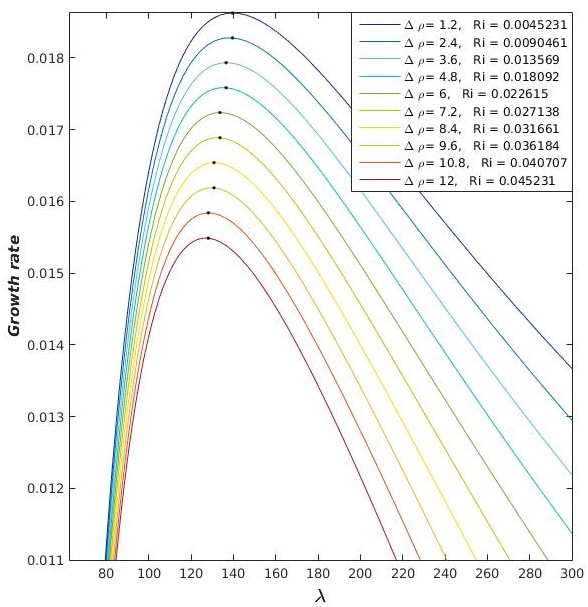
\includegraphics[width=0.75\linewidth]{figures/TG_delatrho.jpg}
\caption[Taylor-Goldstein]{\textit{Prédiction du taux de croissance en fonction de la longueur d'onde d'après la théorie de Taylor-Goldstein pour plusieurs gammes de stratifications}}
	\label{TG_deltarho}
\end{figure}
    \newline
    \textbf{Vitesse} \\
    Le champ de vitesse initiale est : 
    \begin{subequation}
    \begin{align}
        \displaystyle
            \label{u_ini}
            & u(x,y,z,t=0)=U(z)+u'(x,y,z) \\
            \label{v_ini}
            & v(x,y,z,t=0)=v'(x,y,z) \\
            \label{w_ini}
            & w(x,y,z,t=0)=w'(x,y,z)
    \end{align}
    \end{subequation}
    $U(z)$ est le cisaillement vertical de vitesse initial. Il est sous la forme d'une tangente hyperbolique centrée,
    \begin{equation}
        \label{u0_ini}
        U(z)=-tanh(z)
    \end{equation}
    ainsi la couche supérieure va vers la gauche et la couche inférieure vers la droite avec la même vitesse. $u', v'$ et $w'$ sont les petites perturbations nécessaires pour enclencher l'instabilité. Leur forme est choisie pour que le champ de vitesse initiale soit non divergent.
    \begin{subequation}
        \begin{align}
        \displaystyle
            \label{u'_ini}
            & u'(x,y,z)=\epsilon f'(z)\sin{(\frac{2\pi n_x}{L_x}x)}(1+\epsilon_{3D}\sin{(\frac{2\pi n_y}{L_y}y)}) \\
            \label{v'_ini}
            & v'(x,y,z)=0 \\
            \label{w'_ini}
            & w'(x,y,z)=-\epsilon f(z)\frac{2\pi n_x}{L_x}\cos{(\frac{2\pi n_x}{L_x}x)}(1+\epsilon_{3D}\sin{(\frac{2\pi n_y}{L_y}y)})
        \end{align}
    \end{subequation}
    La fonction $f(z)$ localise la perturbation initiale dans la région du cisaillement : 
    \begin{equation}
        f(z)=1-tanh^2(z)
    \end{equation}
    %\[f(z)=1-tanh^2(\frac{z}{\alpha})\]
    %Avec $\alpha=4.29$ et $\epsilon=0.01$
    Avec $\epsilon=0.01$ pour un paramètre sans dimension qui définit l'amplitude de la perturbation dans le sens du courant et $\epsilon_{3D}=0.2$ l'amplitude transverse. $n_x$ et $n_y$ définissent respectivement les longueurs d'ondes dans la direction x et y. 
    \newline
    \textbf{Traceur passif} \\
    Le traceur passif est concentré dans la couche de cisaillement avec une forme :
    \begin{equation}
    \label{phi_ini}
        \phi(x,y,z,t=0)= a\Delta\phi sech^2(az-b)
    \end{equation}
    Avec les constantes $a=1$, qui contrôle l'épaisseur de la couche initiale, et $b=0$, qui contrôle la position de la couche de traceur par rapport au milieu vertical du domaine. 
    
%---Paramètres numériques-----------------------------------------------------    
    \subsection{Paramètres numériques}
    
    Choix de la grille, des pas de temps
    Toutes les simulation présentées ici ont les mêmes condition initiale sur la structure de la densité, d u traceur et du champ de vitesse. Les nombres sans dimensions sont également constant, Ri=0.0045 (sans dimlension ?) et Re=2000. La longueur d'onde sans dimension la plus instable prévu par la théorie de Taylor-Godstein dans ces conditions est $\lambda_{KH}=14.0$. La longueur du domaine est choisie telle que $L_x\approx \lambda_{KH}$ pour n'avoir qu'un seul vortex qui se forme. Les nombres de points de grille ($N_x$, $N_y$ et $N_z$ repectivement dans les directions x, y et z) sont choisit pour avoir une résolution sans dimension isotrope : $\Delta x=\Delta y=\Delta z=0.055$. Les paramètres numériques sont résumés dans le tableau
    \begin{center}
    \begin{tabular}{|c|c|c|c|c|}
    \hline
         Domaine &  Grille & Pas de temps & Pas de temps NBQ & C_s \\ \hline
         L_x = 14.0 & N_x = 256 & & &\\
         L_y = 5.3  & N_y = 96  & \Delta t = 0.006 & N\Delta_{FAST} = 10 & C_s=10 \\
         L_z = 28.6 & N_z = 512 & & & \\
         \hline
    \end{tabular}
    \end{center}
%---Tests numériques----------------------------------------------------------    
    \subsection{Tests numériques}

    kappa net (diffusion implicite+explicite) on ne peut pas descendre les diffusions mol en dessous de la diffusion numérique. \\
    Test vitesse acoustique \\
   
%---Liste des simulations----------------------------------------------------------     
    \subsection{Liste des simulations}

    Variation de krho et kphi


%----------------------------------------------------------------------------------
%%   RESULTATS
%----------------------------------------------------------------------------------

\section{Résultats}

    \subsection{Évolution de la densité et du traceur quand la diffusion moléculaire de la densité varie}
    
    Description de l'évolution de la densité et du traceur pour les configurations.
    Figures des coupes ZX et ZY.
    
    
    \subsection{Évolution de la densité et du traceur quand la diffusion moléculaire du traceur passif varie}
 
    Description de l'évolution de la densité et du traceur pour les configurations.
    Figures des coupes ZX et ZY.
    
    
    \subsection{Diagramme de dispersion}
    
    Description de l'évolution des scatterplots. 
    
    
    \subsection{Évolution macroscopique}
    
    profils réarrangés + issu de la diffusion effective
    K effectif



%----------------------------------------------------------------------------------
%%   DISCUSSION
%----------------------------------------------------------------------------------

\section{Discussion}

Rupture du comportement \\
Détermination de Keff pour le traceur \\
sensibilité à la position \\
différence entre stat en S ou T

%----------------------------------------------------------------------------------
%%   CONCLUSION
%----------------------------------------------------------------------------------

\section{Conclusion}

\bibliographystyle{apalike}
\bibliography{StageM2}
%citep %citet

\end{document}
